\section{Survey of Methods}\label{sec:survey}

Each group covers 1--3 papers; in total at least 5 papers from A/A* conferences or Q1/Q2
journals of the last 3--5 years.

% ---- Template for ONE paper. Copy this call for each paper. ----
\newcommand{\paperbox}[8]{%
  \subsubsection{#1}
  \begin{description}[leftmargin=0pt,style=nextline]
    \item[Reference] #2
    \item[Main idea] #3
    \item[Architecture / method] #4
    \item[Data and key results] #5
    \item[Strengths] #6
    \item[Weaknesses / limitations] #7
    \item[Relevance to this project] #8
  \end{description}
}

\subsection{Group A: Decoding-time Biasing}
Group A leaves the ASR model unchanged. The bias list is compiled into a fast lookup structure
(an FST, a trie or an Aho--Corasick tree) and, during beam search, every hypothesis that follows a path in this
structure receives a bonus score (shallow fusion). The decoding rule is
\begin{equation}\label{eq:sf}
  \hat{y} = \arg\max_{y}\; \log P(y\mid x) + \lambda \log P_C(y),
\end{equation}
where $x$ is the audio, $y$ the sub-word sequence, $P$ the ASR model, $P_C$ the contextual model built from the bias list
and $\lambda$ the biasing weight~\cite{zhao2019}. The list can change per utterance, so no retraining is needed.
We survey two A-ranked Interspeech papers and one recent preprint.

\paperbox{Shallow-Fusion End-to-End Contextual Biasing~\cite{zhao2019}}
  {Zhao et al.\ (Google), Interspeech 2019, pp.~1418--1422, rank A. No official code known to us.}
  {End-to-end models keep only a few candidates in the beam and handle proper nouns poorly, so a biasing phrase is often
   pruned before it can be scored. The paper makes shallow-fusion biasing work for such models and, for the first time
   according to the authors, beats a strong conventional (hybrid) system on contextual tasks.}
  {The bias phrases are compiled into a contextual n-gram WFST and composed with a speller FST that maps sub-word units to words;
   its score is added to the model score as in Eq.~\ref{eq:sf}~\cite{zhao2019}.
   The key changes are: (i) biasing at the \emph{sub-word} level with weight pushing, so that a phrase gains score
   from its first piece and is not pruned early from the beam (instead of rewarding it only at the word end);
   (ii) word-piece units rather than graphemes, which gives sparser matches; (iii) activating a phrase only after
   a context prefix, to avoid over-biasing; (iv) training with extra proper-noun data, including synthetic TTS utterances.
   The biasing step itself needs no training.}
  {Test sets: voice search, songs, contacts (real and TTS) and apps. The abstract reports better results than a conventional
   state-of-the-art model across these tasks~\cite{zhao2019}. \todo{Add 1--2 key WER numbers from the PDF, wrapped in \texttt{\textbackslash authorrep}; the PDF could not be opened when drafting.}}
  {Simple and model-agnostic: the list is swapped at run time without retraining.
   Works with production-scale end-to-end models and established the shallow-fusion recipe used by later work.}
  {Needs a hand-tuned weight $\lambda$ and, for precision, strong context prefixes such as ``call'' or ``play''~\cite{le2021triebias}.
   It matches spellings, not sounds, so it cannot recover a name the model never spells close to the target.
   The paper is from 2019, outside the 3--5 year window; it is included as the milestone of Group A.}
  {Defines the baseline mechanism of Group A and the over-biasing trade-off that every later group tries to avoid.}

\paperbox{Contextualized Streaming End-to-End ASR with Trie-Based Deep Biasing and Shallow Fusion~\cite{le2021triebias}}
  {Le et al.\ (Facebook AI), Interspeech 2021, rank A. Public: the evaluation setup (biasing lists) on LibriSpeech,
   \url{https://github.com/facebookresearch/fbai-speech/tree/master/is21_deep_bias}; no model code is linked in the paper.}
  {Combine three complementary techniques in one streaming RNN-T system, so that rare long-tail words are recognized
   without a large model: a generic WFST for shallow fusion, a trie-based deep biasing module, and a neural language model that also sees the biasing list.}
  {(1) \emph{WFST shallow fusion} applied on word pieces before beam pruning, with dynamic replacement of the bias list and no need for context prefixes.
   (2) \emph{Trie-based deep biasing}: the list becomes a non-trainable trie over word pieces; at each step it outputs a binary vector
   telling which word pieces can start or continue a bias word, and this vector is fed into the RNN-T joiner (DB-RNNT).
   (3) \emph{NNLM contextualization}: the same vector is fed into the neural LM (DB-NNLM, trainable on text only),
   which is shallow-fused with the RNN-T. The final system uses all three.}
  {LibriSpeech with an artificial bias list per utterance (all rare reference words plus $N$ distractors, $N\in\{100,500,1000,2000\}$),
   and in-house video and voice-assistant data. B-WER on test-clean / test-other at $N{=}100$:
   RNN-T baseline \authorrep{14.1}/\authorrep{30.6}, WFST only \authorrep{9.4}/\authorrep{22.2}, final system \authorrep{5.7}/\authorrep{14.1};
   at $N{=}2000$ the final system gets \authorrep{7.3}/\authorrep{18.9}.
   DB-NNLM gives \authorrep{19.5\%} average relative B-WER gain over WFST + DB-RNNT. On in-house data the final system improves
   over a hybrid baseline by \authorrep{5.4\%}--\authorrep{9.3\%} with a model of about 200~MB instead of 4~GB (8-bit quantized).
   U-WER stays almost unchanged.}
  {Streaming; strong, complementary gains; no retraining for a new list; small footprint; releases the biasing-list protocol, which makes B-WER/U-WER comparisons reproducible.}
  {Deep biasing (DB-RNNT, DB-NNLM) was trained with only 400--800 distractors and degrades on much longer lists;
   trie-based deep biasing alone is weaker than WFST shallow fusion; the NNLM gain is smaller on in-house data;
   no model code is linked in the paper. At 5 years old it is at the edge of the 3--5 year window.}
  {Provides the B-WER/U-WER protocol and the list-size effect that our dictionary-size ablation on CopyNE also probes.}

\paperbox{TurboBias: Universal ASR Context-Biasing powered by GPU-accelerated Phrase-Boosting Tree~\cite{andrusenko2025turbobias}}
  {Andrusenko et al.\ (NVIDIA), 2025. arXiv preprint (the arXiv comments say ASRU 2025; ASRU is unranked), so it does \emph{not} count toward the survey threshold. Code: NeMo toolkit.}
  {Shallow-fusion phrase boosting that is fast on GPU and works with CTC, RNN-T and attention encoder--decoder (AED) models alike, even with up to 20K phrases.}
  {An Aho--Corasick prefix tree is built over the tokenized phrases with backoff (failure) links and a modified weight rule:
   a non-root arc at depth $d>1$ gets bonus $c_0\beta+\ln d$ (example $c_0{=}1$, $\beta{=}2$) instead of a uniform reward at the final node.
   The tree is stored as a GPU table (adapted from NGPU-LM) queried over the whole vocabulary,
   with a Triton kernel so that CUDA graphs can be used. For AED the end-of-sequence score is raised to avoid truncating a phrase.}
  {FastConformer CTC / RNN-T (114M) / AED (179M) models trained on 24K hours of English; test sets Earnings21, MultiMed and CSTalks.
   On CSTalks with RNN-T beam search the phrase F-score goes from \authorrep{44.2} to \authorrep{82.9} and WER from \authorrep{12.8} to \authorrep{9.6}.
   The speed cost is about \authorrep{2--5\%} RTFx. With 20K phrases the F-score is \authorrep{78.4}\% and WER \authorrep{11.42}\%.}
  {One framework for all major model types; negligible slowdown; scales to thousands of phrases; open source.}
  {Preprint only. English only, one GPU type and one model scale; beam search is offline;
   greedy decoding can hurt words outside the list; boosting weights are tuned on development sets.}
  {Shows how far shallow fusion has been pushed in engineering terms; used as a reference, not as a counted paper.}

\subsection{Group B: Dedicated Biasing Modules}
\paperbox{\todo{CLAS}~\cite{pundak2018}}
  {\todo{}}{\todo{}}{\todo{}}{\todo{}}{\todo{}}{\todo{}}{\todo{}}
\paperbox{CopyNE~\cite{lin2024copyne}}
  {ACL 2024 (A*), \todo{}}{\todo{}}{\todo{}}{\todo{}}{\todo{}}{\todo{}}{\todo{candidate for demo/ablation}}

\subsection{Group C: Post-recognition Correction}
\paperbox{CTC-based Word Spotter~\cite{andrusenko2024ctcws}}
  {Interspeech 2024, \todo{}}{\todo{}}{\todo{}}{\todo{}}{\todo{}}{\todo{}}{\todo{candidate for demo/ablation}}

\subsection{Group D: Bias Retrieval}

\subsubsection{BR-ASR: Efficient and Scalable Bias Retrieval Framework for Contextual Biasing ASR in Speech LLM}
BR-ASR~\cite{gong2025brasr} was presented by Gong et al.\ at Interspeech 2025 (rank A, pp.~4043--4047) and belongs to
Group D1 (bias retrieval). The authors do not release code.

\paragraph{Problem.} A speech LLM can use a list of rare words (names, product terms) if the list is written in its prompt.
But a long list does not scale: Prompt-Qwen-Audio already collapses at 500 words (B-WER \authorrep{32.1}/\authorrep{39.1}).
We need to pick a short list of likely words for each utterance.

\paragraph{Key idea.} BR-ASR \emph{retrieves first, then decodes}. A small retriever listens to the whole utterance, turns it into one vector,
and finds the bias words whose vectors are closest. Only these top-$K$ words go into the prompt (Fig.~\ref{fig:brasr}).
The retriever is trained so that speech and words live in one shared space, and it is separate from the speech LLM, so the LLM is never retrained.
In short, the paper's three novelties are:
\begin{itemize}
  \item retrieval works directly from audio, using the speech LLM's own frozen encoders;
  \item a homophone curriculum trains the retriever to tell similar-sounding words apart;
  \item the list can reach 200k words by updating an index, with no fine-tuning.
\end{itemize}

\begin{figure}[h]
\centering
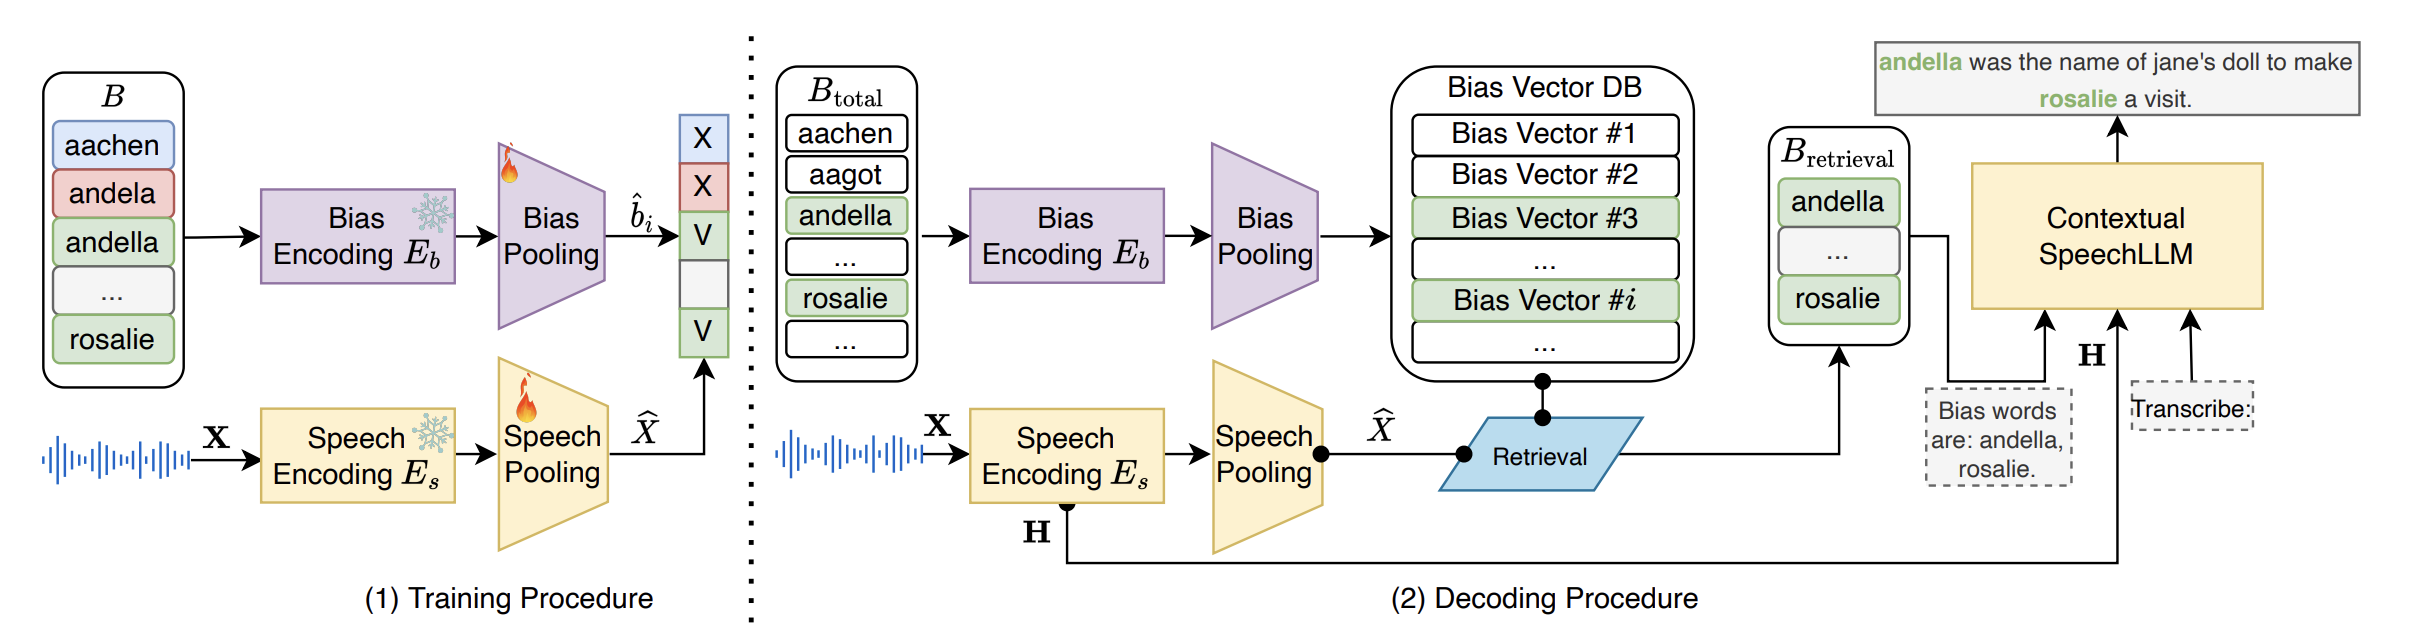
\includegraphics[width=\linewidth]{TV4_D1_BR-ASR_pipeline.png}
\caption{BR-ASR pipeline~\cite{gong2025brasr} (snowflake: frozen, flame: trainable).
\textbf{(1) Training:} an utterance $X$ and bias words $B$ (correct words V, random and homophone negatives X) are encoded by frozen
encoders $E_s$, $E_b$ and pooled by two trainable blocks into one vector $\hat X$ and one vector $\hat b_i$ per word;
a contrastive loss pulls $\hat X$ toward the correct words and away from the wrong ones, including near-homophones such as
``andela'' vs.\ ``andella''. \textbf{(2) Decoding:} the full list $B_{\mathrm{total}}$ is encoded once offline into a Bias Vector DB;
for each utterance, retrieval returns $B_{\mathrm{retrieval}}$, which is given to the contextual SpeechLLM as a text prompt
together with the speech features $H$ to produce the transcript.}\label{fig:brasr}
\end{figure}

\paragraph{How it works, in three steps.}
\begin{enumerate}
  \item \textbf{Train a small retriever (once).}
    The speech encoder $E_s$ is the frozen encoder of the speech LLM. Each bias word is also encoded by a frozen encoder $E_b$:
    \emph{AcousticBias} synthesizes the word with TTS and passes it through $E_s$, while \emph{TextualBias} uses the text side of the LLM,
    which works better because it avoids the gap between synthetic and real speech.
    Two trainable attention-pooling blocks then turn the speech features into one vector $\hat X$ and each word into one vector $\hat b_i$.
    A CLAP-style contrastive loss with a learnable temperature pulls $\hat X$ toward the correct words and away from wrong ones.
    Hard negatives come from a \emph{homophone curriculum}: words whose phoneme sequences (G2P) differ from a correct word by at most 2 edits,
    mixed in at a share that grows from 1\% to 50\% on a sigmoid schedule, so training goes from easy to hard.
  \item \textbf{Index the bias list (once per domain).}
    All words of $B_{\mathrm{total}}$ (up to 200k) are encoded, normalized and stored in a FAISS inner-product index. Changing the list only means updating the index.
  \item \textbf{Retrieve and decode (for every utterance).}
    The utterance vector $\hat X$ queries the index and returns the top-$K$ words. The contextual SpeechLLM (Qwen-Audio or SLAM-ASR)
    receives them in the prompt ``Bias words are: \dots'' together with the speech features $H$, and writes the transcript.
\end{enumerate}

\paragraph{Why it is different.} Earlier filters such as CTC-filter select words from a first-pass hypothesis, so a word missing from the N-best list can never be recovered.
BR-ASR searches with the audio itself. Compared with RECAST, it uses one vector per utterance, which is simple and fast but loses the position of a word.

\paragraph{Contributions.} Each contribution below is linked to the result it improves (Table~\ref{tab:brasr}).
\begin{enumerate}
  \item \textbf{Audio-to-word contrastive retrieval.} Candidates are retrieved from the speech itself, using the frozen encoders of the speech LLM, instead of from a CTC hypothesis.
    This avoids the irrecoverable error of CTC-filter when the correct word is missing from the N-best list, and it replaces a long prompt by a short one.
    \emph{Effect:} at $N{=}2000$, B-WER on test-clean/other falls from \authorrep{8.4}/\authorrep{18.4} (no bias) to \authorrep{2.8}/\authorrep{7.1},
    better than the previous best, USTR-CT (\authorrep{3.0}/\authorrep{7.6}), while WER also improves.
  \item \textbf{Dynamic homophone curriculum.} Hard negatives from near-sounding words are introduced with increasing difficulty on a sigmoid schedule, so the retriever learns to separate words that sound alike.
    \emph{Effect:} on test-other, homophone confusions in the top-50 fall from \authorrep{91.3\%} to \authorrep{58.4\%}, and B-WER improves from \authorrep{7.9} to \authorrep{7.1}.
  \item \textbf{Decoupled, plug-and-play retrieval.} Because retrieval is separate from decoding, the ASR model is not retrained, words are added or removed by updating the index,
    and the same retriever fits several backbones.
    \emph{Effect:} growing the list from 2k to 200k words raises B-WER only from \authorrep{9.9} to \authorrep{12.8}, at \authorrep{20\,ms} per query on an RTX~4090.
\end{enumerate}

\begin{table}[h]
\centering\footnotesize
\begin{tabularx}{\textwidth}{@{}l X c c@{}}
\toprule
\textbf{Contribution} & \textbf{Setting} & \textbf{WER} & \textbf{B-WER} \\
\midrule
Baseline & Qwen-Audio, no bias & \authorrep{2.0}/\authorrep{4.2} & \authorrep{8.4}/\authorrep{18.4} \\
Audio retrieval & Prompt-Qwen-Audio + BR, $N{=}2000$ & \authorrep{1.2}/\authorrep{2.8} & \authorrep{2.8}/\authorrep{7.1} \\
Prior SOTA & USTR-CT, $N{=}2000$ & \authorrep{2.2}/\authorrep{5.8} & \authorrep{3.0}/\authorrep{7.6} \\
\midrule
No curriculum & Textual, attn.\ pooling (other) & \authorrep{3.0} & \authorrep{7.9} \\
Curriculum & Textual, attn.\ pooling (other) & \authorrep{2.8} & \authorrep{7.1} \\
\midrule
Scale & BiasEncoder-Qwen-Audio, 2k $\to$ 200k (other) & -- & \authorrep{9.9}$\to$\authorrep{12.8} \\
\bottomrule
\end{tabularx}
\caption{Key results of BR-ASR on LibriSpeech (test-clean/test-other unless marked; all numbers author-reported). With the curriculum, homophone recall in the top-50 drops from
\authorrep{91.3\%} to \authorrep{58.4\%} (lower is better). Retrieval over 200k entries takes \authorrep{20\,ms} on an RTX~4090.}\label{tab:brasr}
\end{table}

\paragraph{Discussion.} BR-ASR scales to very large lists at low latency and improves three different backbones, but it has limits.
One vector per utterance must be close to several words and loses position information, and the paper does not analyze multi-word sentences.
Evaluation uses only LibriSpeech with random rare-word distractors, hard negatives come only from the bias list itself, and on SLAM-ASR the gain over
CTC-filter is small (B-WER \authorrep{4.2}/\authorrep{9.3} vs.\ \authorrep{4.4}/\authorrep{10.0}).

\subsubsection{RECAST: Retrieval-Augmented Contextual ASR via Decoder-State Keyword Spotting}
RECAST~\cite{mittal2025recast} was presented by Mittal, Sarawagi and Jyothi in Findings of EMNLP 2025 (rank A*, pp.~3780--3793)
and belongs to Group D1 (bias retrieval). Code: \texttt{github.com/}\allowbreak\texttt{AshishMittal/}\allowbreak\texttt{Recast}.

\paragraph{Problem.} Contextual biasing gives the recognizer a list of rare words (names, places, drug names) that may appear in the audio.
With thousands of words the list is too long for a prompt, and a long list makes the model worse, not better.
We therefore need to pick a short list of likely words for each utterance.

\paragraph{Key idea.} RECAST \emph{retrieves first, then decodes}, like BR-ASR, but it asks the question in a different way.
At every step the Whisper decoder already ``knows'' which part of the audio it is listening to, because of cross-attention.
RECAST reads this decoder state and uses it as a search query: ``which keyword tokens sound like what I am hearing now?''
Matching tokens are then joined back into whole keywords, and the best $\mathcal{K}$ keywords are put into the Whisper prompt (Fig.~\ref{fig:recast}).
Whisper itself is never changed, and no recording of the keywords is needed.

\begin{figure}[h]
\centering
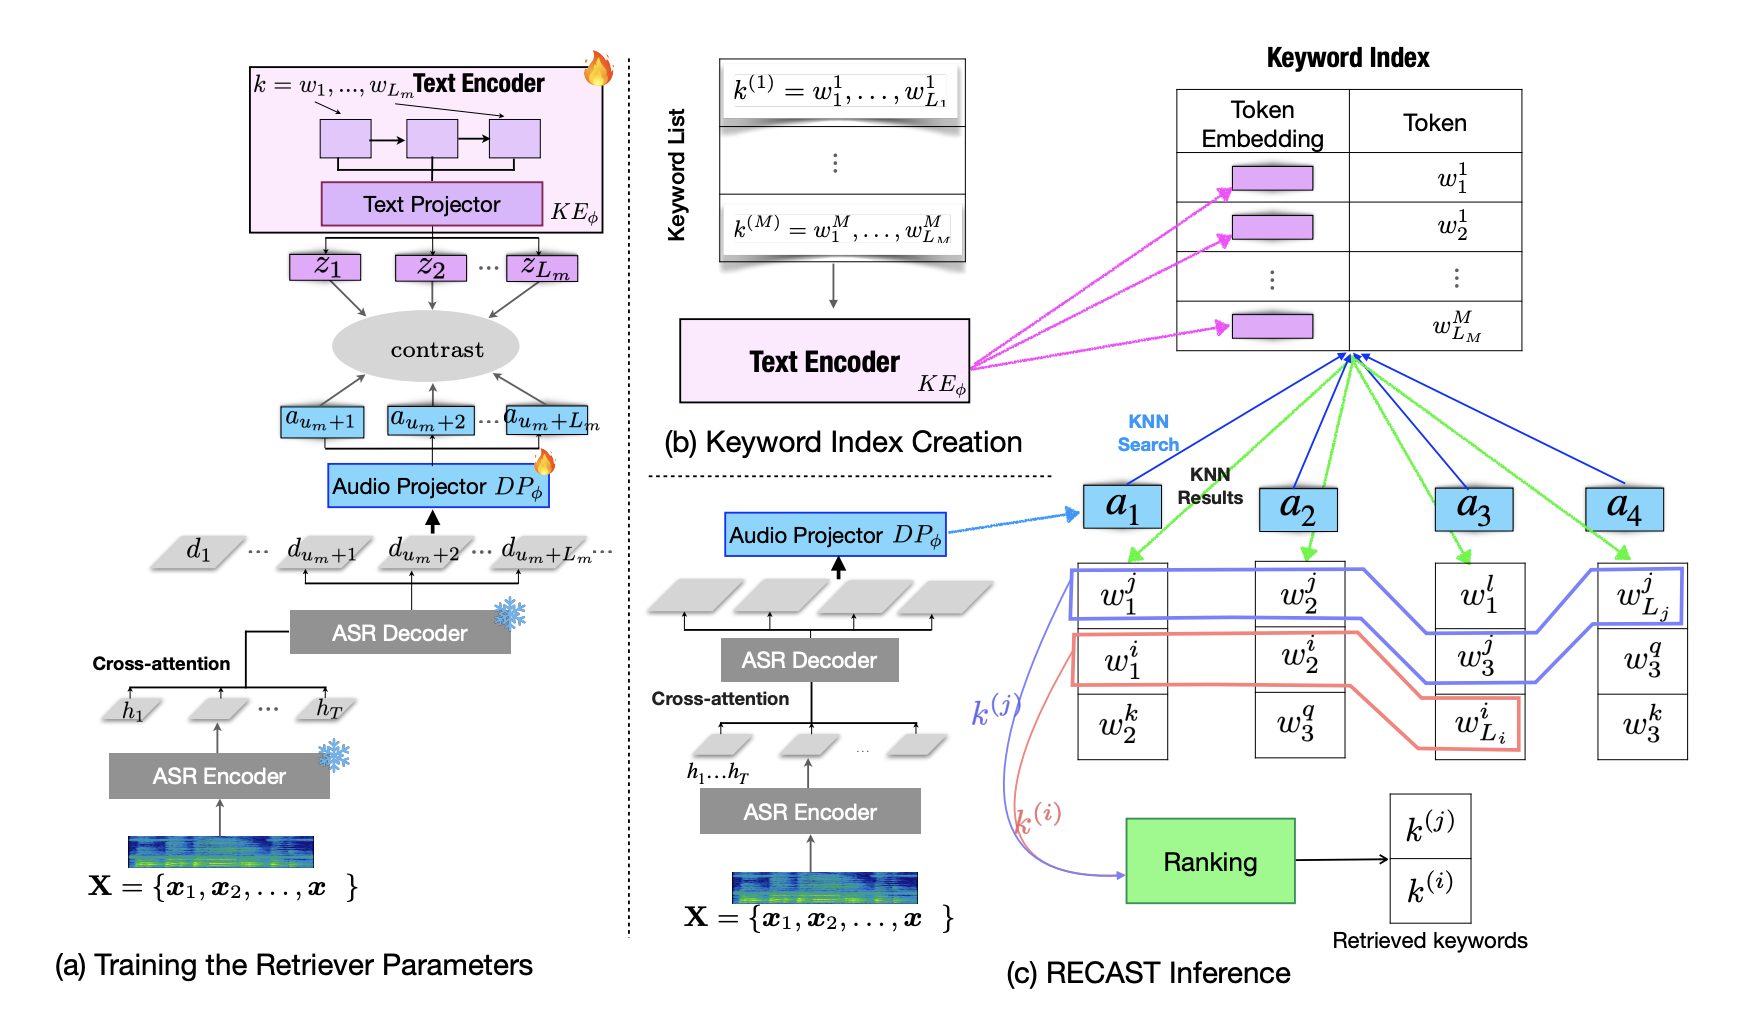
\includegraphics[width=\linewidth]{TV4_D1_RECASE_pipeline.png}
\caption{RECAST pipeline~\cite{mittal2025recast} (snowflake: frozen, flame: trainable).
\textbf{(a) Training:} the keyword encoder $\mathrm{KE}_\phi$ turns the tokens of a keyword into contextual embeddings $z_\ell$, and the audio projector
$\mathrm{DP}_\phi$ turns the frozen decoder states at the same tokens into $a_\ell$; a contrastive loss aligns each $a_\ell$ with its $z_\ell$.
\textbf{(b) Indexing:} every keyword in the list is encoded once and its token embeddings are stored in a kNN index.
\textbf{(c) Inference:} at each decoding step, $a_t$ queries the index; consecutive token matches are chained into keyword spans
(blue and red paths), and a ranker returns the top-$\mathcal{K}$ keywords.}\label{fig:recast}
\end{figure}

\paragraph{How it works, in three steps.}
\begin{enumerate}
  \item \textbf{Train a small retriever (once, on LibriSpeech only).}
    Two small networks are added next to the frozen Whisper (6.5M parameters in total):
    a keyword encoder $\mathrm{KE}_\phi$ (an LSTM that reads the subword tokens of a keyword from left to right)
    and an audio projector $\mathrm{DP}_\phi$ (a feed-forward layer applied to the decoder state).
    Both map into the same 512-dimensional space. Training is contrastive: the decoder state at the moment a token is spoken
    must be close to the text embedding of that token and far from other tokens.
    The hardest negatives are the same token with a different left context, so the retriever learns to use the preceding tokens, not just the token itself.
  \item \textbf{Index the keyword list (once per domain).}
    Every keyword is split into tokens, encoded by $\mathrm{KE}_\phi$, and each token embedding is stored in a kNN index together with
    the keyword it belongs to and its position in that keyword. No audio and no retraining are needed to change the list.
  \item \textbf{Retrieve and rank (for every utterance).}
    While Whisper decodes greedily, each decoder state is projected by $\mathrm{DP}_\phi$ and used to fetch its $\hat{\mathcal{T}}$ nearest token embeddings.
    A keyword is followed from one step to the next: if its next token appears among the neighbours, the hypothesis moves on; if not, it gets one error
    (at most $E_{\max}$ are allowed, to absorb tokenization differences). Finished keywords are ranked by their average similarity, boosted for longer keywords
    (so longer, more informative words win), and keywords from different positions in the utterance are preferred. The top-$\mathcal{K}$ go into the prompt.
\end{enumerate}
In words, the training objective rewards the retriever when the decoder state at the moment a token is spoken is closer to that token's text embedding
than to every other token, including the hard negatives. Keywords for training are taken automatically from the transcripts with KeyBERT.

\paragraph{Why it is different.} BR-ASR compresses the whole utterance into one vector; RECAST keeps one query per decoding step, so it knows \emph{where} a keyword is.
Phonetic baselines (Soundex, Metaphone) and BM25 match the first-pass \emph{text} of Whisper, so they fail when that text is already wrong;
RECAST searches with the decoder state instead.

\paragraph{Contributions.} Each contribution is linked to the result it improves (Tables~\ref{tab:recast} and~\ref{tab:recast-abl}).
\begin{enumerate}
  \item \textbf{Decoder-state contrastive retriever.} Audio and text tokens are aligned in a shared space using the ASR decoder itself, with no keyword audio and no change to the backbone.
    \emph{Effect:} with $\hat{\mathcal{T}}{=}20$ it beats Soundex, Metaphone, Double Metaphone, NYSIIS and BM25, as well as WFST rescoring and PRISM;
    on Location (small), Recall@50 is \authorrep{82.5} against \authorrep{75.0} for Double Metaphone, and E-WER is \authorrep{17.2} against \authorrep{20.3}.
  \item \textbf{Token-level tracking and ranking.} Matching subword tokens and chaining them into spans tolerates tokenization mismatches, and the length-scaled, position-diverse ranker selects the shortlist.
    \emph{Effect:} scaled distance plus positional diversity lowers E-WER on Location (small) from \authorrep{18.6} to \authorrep{17.2} (Table~\ref{tab:recast-abl}).
  \item \textbf{Generalization across domains, models and languages.} The retriever is trained only on LibriSpeech, yet works on four out-of-domain sets with up to 4{,}000 keywords,
    on Hindi, and with Phi-4 and GPT-4o-mini.
    \emph{Effect:} the real-time factor stays between \authorrep{0.013} and \authorrep{0.015} from 1k to over 4k keywords.
\end{enumerate}

\begin{table}[h]
\centering\footnotesize
\begin{tabularx}{\textwidth}{@{}l X c c@{}}
\toprule
\textbf{Row} & \textbf{Setting} & \textbf{Recall@50} & \textbf{WER / E-WER} \\
\midrule
Baseline & Whisper large-v2, Location (small) & \authorrep{53.7} & \authorrep{19.6}/\authorrep{37.7} \\
Phonetic & Double Metaphone, Location (small) & \authorrep{75.0} & \authorrep{12.9}/\authorrep{20.3} \\
Retriever & RECAST $\hat{\mathcal{T}}{=}20$, Location (small) & \textbf{\authorrep{82.5}} & \textbf{\authorrep{11.5}/\authorrep{17.2}} \\
\midrule
Baseline & Whisper large-v2, Drugs & \authorrep{16.1} & \authorrep{16.5}/\authorrep{74.8} \\
Retriever & RECAST $\hat{\mathcal{T}}{=}20$, Drugs & \authorrep{55.3} & \authorrep{12.3}/\authorrep{49.6} \\
\midrule
Baseline & Whisper, LibriSpeech test-other, 1k distractors & \authorrep{79.5} & \authorrep{6.7}/\authorrep{10.6} \\
Retriever & RECAST $\hat{\mathcal{T}}{=}20$, test-other & \authorrep{88.0} & \authorrep{5.4}/\authorrep{7.8} \\
\bottomrule
\end{tabularx}
\caption{Key results of RECAST (all numbers author-reported). Location and Drugs belong to the entity-rich PRISM benchmark;
the downstream model is Whisper large-v2 with the retrieved keywords in the prompt.}\label{tab:recast}
\end{table}

\begin{table}[h]
\centering\footnotesize
\begin{tabularx}{\textwidth}{@{}l X c c@{}}
\toprule
\textbf{Ablation} & \textbf{Variant} & \textbf{Location (small) E-WER} & \textbf{Drugs Recall@50} \\
\midrule
Ranker & average distance & \authorrep{18.6} & -- \\
Ranker & scaled distance + positional diversity & \textbf{\authorrep{17.2}} & -- \\
\midrule
Hard negatives & $\mathcal{N}{=}0$ & \authorrep{18.3} & \authorrep{40.20} \\
Hard negatives & $\mathcal{N}{=}10$ & \textbf{\authorrep{17.2}} & \textbf{\authorrep{55.34}} \\
\bottomrule
\end{tabularx}
\caption{Ablations of RECAST (author-reported). Hard negatives matter most on Drugs, where phonetically similar distractors are common.}\label{tab:recast-abl}
\end{table}

\paragraph{Discussion.} RECAST scales to thousands of keywords at near-constant latency, needs no keyword audio, and transfers to Hindi, where
phonetic baselines do not apply (E-WER falls by \authorrep{12.7\%} at $E_{\max}{=}2$ and \authorrep{19.5\%} at $E_{\max}{=}3$). Selecting a short list also protects LLMs:
Phi-4 with $\mathcal{K}{=}50$ hallucinates and raises WER, whereas $\mathcal{K}{=}10$ helps.
The authors list three limits: it needs an encoder--decoder ASR model (CTC and RNN-T have no comparable decoder states),
it is a two-pass pipeline, and it is tested only up to 4k keywords.
In addition, on the Names set it only matches the best phonetic baseline in recall, and Vietnamese is not evaluated, so its subword tokenization may behave differently, as the authors observe for Hindi.

\subsection{Comparison}
\begin{table}[h]
\centering\small
\begin{tabularx}{\textwidth}{@{}l l l X X X@{}}
\toprule
\textbf{Paper} & \textbf{Group} & \textbf{Venue/Year} & \textbf{Needs training?} & \textbf{Streaming?} & \textbf{Main pros/cons} \\
\midrule
Zhao et al.~\cite{zhao2019} & A & Interspeech 2019 & No (FST built per list) & \todo{check in PDF} & Simple, model-agnostic; needs tuned $\lambda$ and context prefixes \\
Le et al.~\cite{le2021triebias} & A & Interspeech 2021 & Deep biasing: yes; WFST: no & Yes & Strong and small, but deep biasing degrades on long lists \\
\todo{} & & & & & \\
\bottomrule
\end{tabularx}
\caption{Comparison of the surveyed methods.}\label{tab:survey}
\end{table}
